\documentclass[aspectratio=169]{beamer}
\usetheme{metropolis} % Use metropolis theme

\usepackage[ngerman]{babel}
\usepackage{amsmath}
\usepackage{amssymb}
\usepackage{mathtools}
\usepackage{graphicx}
% \usepackage{raleway}

\title{Rolling-bouncing ball - Dynamik eines Balles}
\author{Helene Rößler, Norbert Hammer}
\date{}


\begin{document}
\maketitle

\section{Bewegungsgleichungen}

\begin{frame}{Massepunkt auf einer Kurve}
\begin{itemize}
    \item Ball als Massepunkt modelliert
    \item Bewegung auf Kurve gegeben durch $G(q)=0$
    \item Lösungskurve $q(t)$
    \item Das Variationsprinzip
    \begin{equation*}
        0 = \delta \int_0^T L(q, \dot{q}) \boldsymbol{ + \lambda G(q)} \ dt
    \end{equation*}
    \item führt zu
        \begin{align*}
            m \ddot{q} &= F + \lambda \nabla G(q)\\
            0 &= G(q).
        \end{align*}
\end{itemize}
\end{frame}

\begin{frame}{Massepunkt auf einer Kurve}
\begin{itemize}
    \item In zweiten Ableitungen ausgedrückt:
        \begin{equation*}
        \underbrace{
        \begin{pmatrix}
          m & 0 & 0 \\
          0 & m & 0 \\
          0 & 0 & 0
        \end{pmatrix}}_{\eqcolon M ~ \text{(Massenmatrix)}}
        \begin{pmatrix} \ddot{q} \\ \ddot{\lambda} \end{pmatrix} =
        \begin{pmatrix}
          F + \lambda \nabla G(q)\\
          G(q)
        \end{pmatrix}
        \end{equation*}
        Anmerkung: $\ddot{q}, F + \lambda \nabla G(q) \in \mathbb{R}^2$
\end{itemize}
\end{frame}

\begin{frame}{Massepunkt im freien Fall}
\begin{itemize}
    \item ohne Nebenbedingung $G(q)=0$
    \item Das Obige wird zu
        \begin{equation*}
            F = \begin{pmatrix}
            m & 0 \\
            0 & m
            \end{pmatrix} \ddot{q}.
        \end{equation*}
\end{itemize}
\end{frame}

\section{Krümmung einer impliziten Kurve}

\begin{frame}{Krümmung einer Kurve}
\begin{itemize}[<+->]
    \item Sei $\varphi (t)$ Parameterdarstellung einer Kurve.
    \item<.-> Krümmung ist gegeben durch
        \begin{equation*}
        \kappa = \frac{\varphi_1'(t) \varphi_2''(t) - \varphi_2'(t) \varphi_1''(t)}{\| \varphi '(t) \|^3}.
        \end{equation*}
    \item Problem: Wir kennen $\varphi$ nicht!
    \item<.-> Beachten Sie: $\kappa$ nicht von Wert von $\varphi$ abhängig,
        nur von Ableitungen
    \item<.-> Lösung des Problems: Hauptsatz über implizite Funktionen
\end{itemize}
\end{frame}

\begin{frame}{Krümmung einer Kurve}
\begin{itemize}[<+->]
    \item Hauptsatz liefert erste (und damit auch zweite) Ableitung von Funktion,
        die mit Kurve übereinstimmt
    \item Problem: Kurve muss lokal als Funktion darstellbar sein
    \item Lösung:

    \begin{tabular}[t]{l c}
    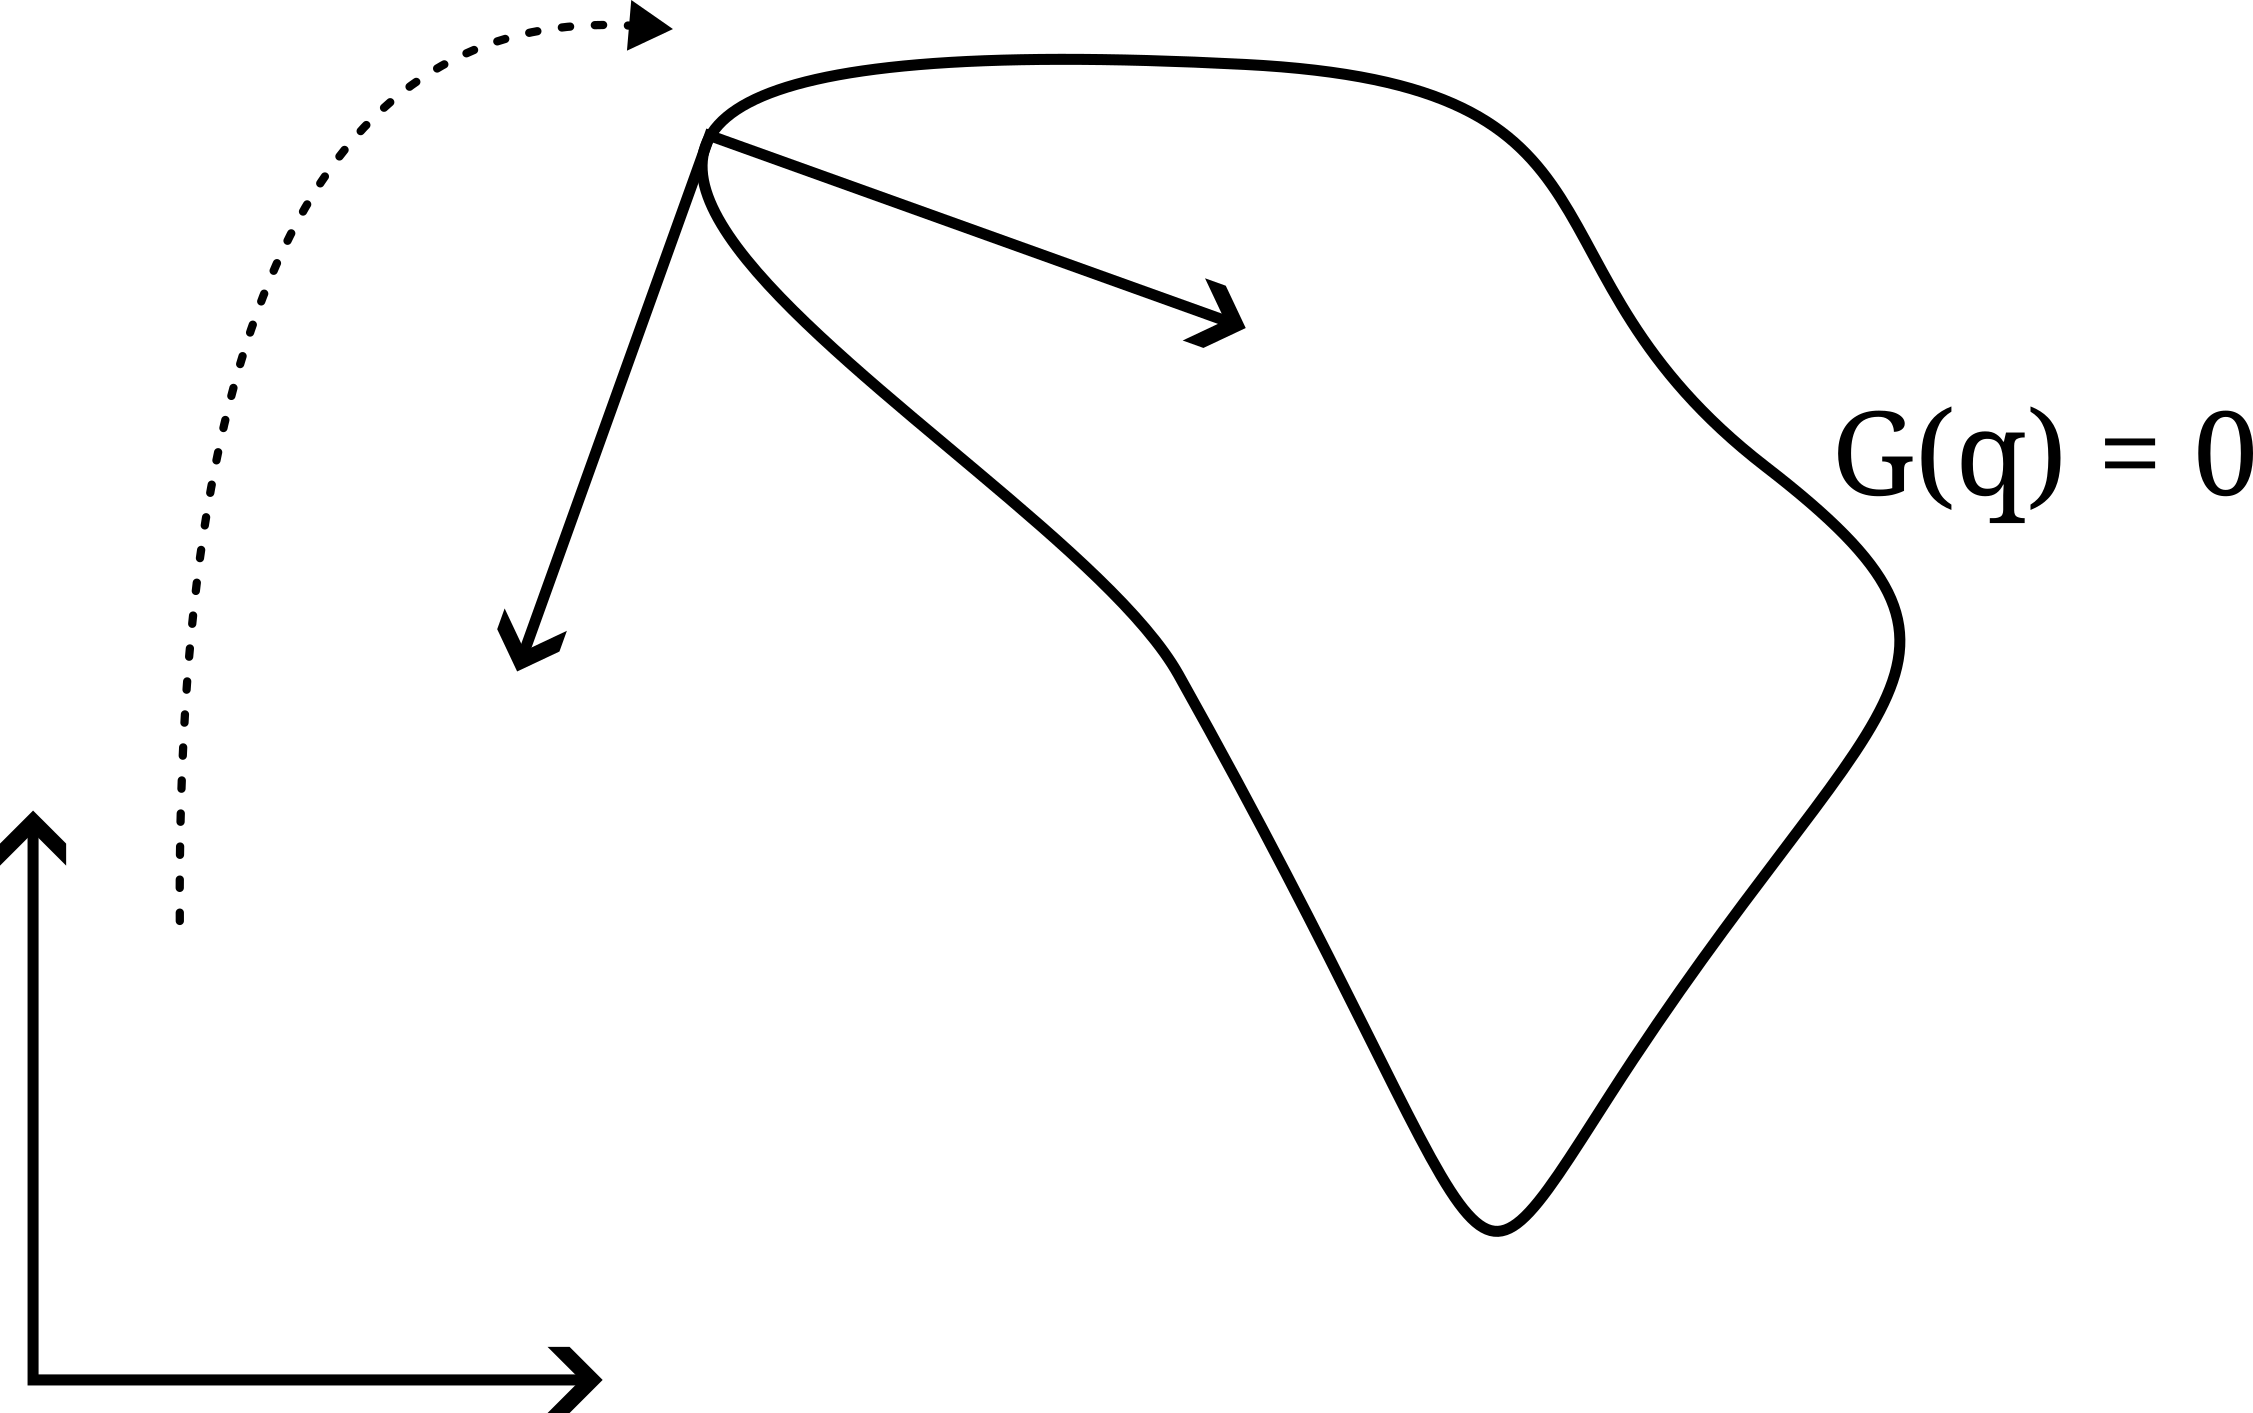
\includegraphics[scale=0.7]{./trafo.png} &
    {$\!\begin{aligned} % http://tex.stackexchange.com/q/98482/16595
        \nu &= \frac{ \nabla G(x_0) }{ \| \nabla G(x_0) \| } \\
        \tau &= (-\nu_2, \nu_1)
        \end{aligned}$}
    \end{tabular}
\end{itemize}
\end{frame}

\begin{frame}{Krümmung einer Kurve}
\begin{itemize}
    \item Krümmung des Graphen der Funktion $f(t)$:
        \begin{equation*}
        \kappa = \frac{f''(t)}{(1 + f'(t)^2)^{3/2}}.
        \end{equation*}
\end{itemize}
\end{frame}


\section{Newmark-Verfahren}

\begin{frame}{Allgemeine Form}
Ausgangssituation ist eine Bewegungsgleichung der Form:
\begin{equation*}
	F = M \ddot{x} + C \dot{x} + Kx
\end{equation*}

\begin{itemize}
	\item $x(t) \in \mathbb{R}^{m}$: Ortsvektor
	\item $M, C, K \in \mathbb{R}^{m \times m}$: Massen-, Dämpfungs- und Steifigkeitsmatrix
\end{itemize}
\end{frame}

\begin{frame}{Allgemeine Form}

\begin{itemize}
\item Ausgangswerte zum Zeitpunkt $t_n$
\begin{align*}
	x_n, \quad v_n := \dot{x}_n, \quad a_n := \ddot{x}_n.
\end{align*}
\item Näherung für $t_{n+1} = t_n + h$ ist allgemein gegeben durch:
\begin{align*}
	F_{n+1} &= M a_{n+1} + C v_{n+1} + K q_{n+1}\\
	v_{n+1} &= v_{n} + h\left({\left(1 - \gamma\right) a_{n} + \gamma{a_{n+1}}}\right)\\
	x_{n+1} &= x_{n} + h v_{n} + \frac{h^2}{2} \left({\left(1 - 2\beta\right) a_{n} + 2\beta a_{n+1}}\right)
\end{align*}
\end{itemize}

\end{frame}


\begin{frame}{Spezialfall}
\begin{itemize}
	\item  $\beta = \frac{1}{4}, \gamma = \frac{1}{2}$ $\Rightarrow$ quadratische Genauigkeit
	\item $K = \mathbf{0} \in \mathbb{R}^{m \times m}$
\end{itemize}
Führt zu
\begin{align*}
	F(x_{n+1}) &= M a_{n+1} + C v_{n+1}\\
	v_{n+1} &= v_n + \frac{h}{2} (a_n + a_{n+1})\\
	x_{n+1} &= x_n + h v_n + \frac{h^2}{4} (a_n + a_{n+1}).
\end{align*}
\end{frame}

\begin{frame}{Setup für die ODE}
\textbf{Fall:} Ball befindet sich in der Flugphase\\
\pause
\vspace{0.3cm}
	\begin{itemize}
		\item Dämpfung: $C = \mathbf{0} \in \mathbb{R}^{2 \times 2}$
		\item Massenmatrix:
		\[
		M =
		\begin{pmatrix}
			m & 0 \\
			0 & m
		\end{pmatrix}
		\]
		\item Kraftvektor (Gravitation): \quad $F = m g$
		\item Anfangswerte: $x_0, v_0$ und $a_0$ werden vom Algorithmus direkt als aktueller Zustand des Balls übernommen.
	\end{itemize}
\end{frame}

\begin{frame}{Setup für die DAE}
\textbf{Fall:} Ball befindet sich in der Rollphase\\
\pause
\vspace{0.3cm}
\begin{itemize}
	\item Dämpfung (durch Dämpfungsfaktor $c \in \mathbb{R}$) und Masse:
	\begin{equation*}
		C :=
		\begin{pmatrix}
			c & 0 & 0\\
			0 & c & 0\\
			0 & 0 & 0
		\end{pmatrix},
		\quad
		M =
		\begin{pmatrix}
			m & 0 & 0 \\
			0 & m & 0 \\
			0 & 0 & 0
		\end{pmatrix}
	\end{equation*}
	\item Kraftvektor:
	\[F =
	\begin{pmatrix}
		mg + \lambda \nabla G(q)\\
		G(q)
	\end{pmatrix}.
	\]
\end{itemize}
\end{frame}

\begin{frame}{Setup für die DAE}
Anfangswerte:
\begin{itemize}
	\item $x_0$: aktuelle Position des Balls
	\item $v_0$: liegt tangential zur Kurve
	\item $a_0$: Formel für Beschleunigung entlang einer Kurve:
	\[
	a_0 = a \tau + \kappa \| v_0 \|^2 \nu
	\]

	\qquad mit Tangentialvektor $\tau$, Normalvektor $\nu$ und\\
	\qquad Krümmung der Bahn $\kappa$:

	\item kein Startwert für $\lambda$ benötigt
\end{itemize}
\end{frame}

\section{Zentrifugalkraft}

\begin{frame}{Zentrifugalkraft auf einer allgemeinen Kurve}
\begin{itemize}
\item Wir wissen aus dem Kapitel über Newmark:
    \begin{equation*}
        \mathbf{a} = \textcolor{lightgray}{ a \tau + } \kappa \| v \|^2 \nu
    \end{equation*}
\item Also:
        \begin{equation*}
            F_c \coloneq m \| v \|^2 \kappa
        \end{equation*}
\item Normalkraft durch Bewegung auf Kurve; stimmt auf Kreis mit Zentrifugalkraft
        überein
\end{itemize}
\end{frame}

\section{Zustandswechsel}

\begin{frame}{graphisch}
	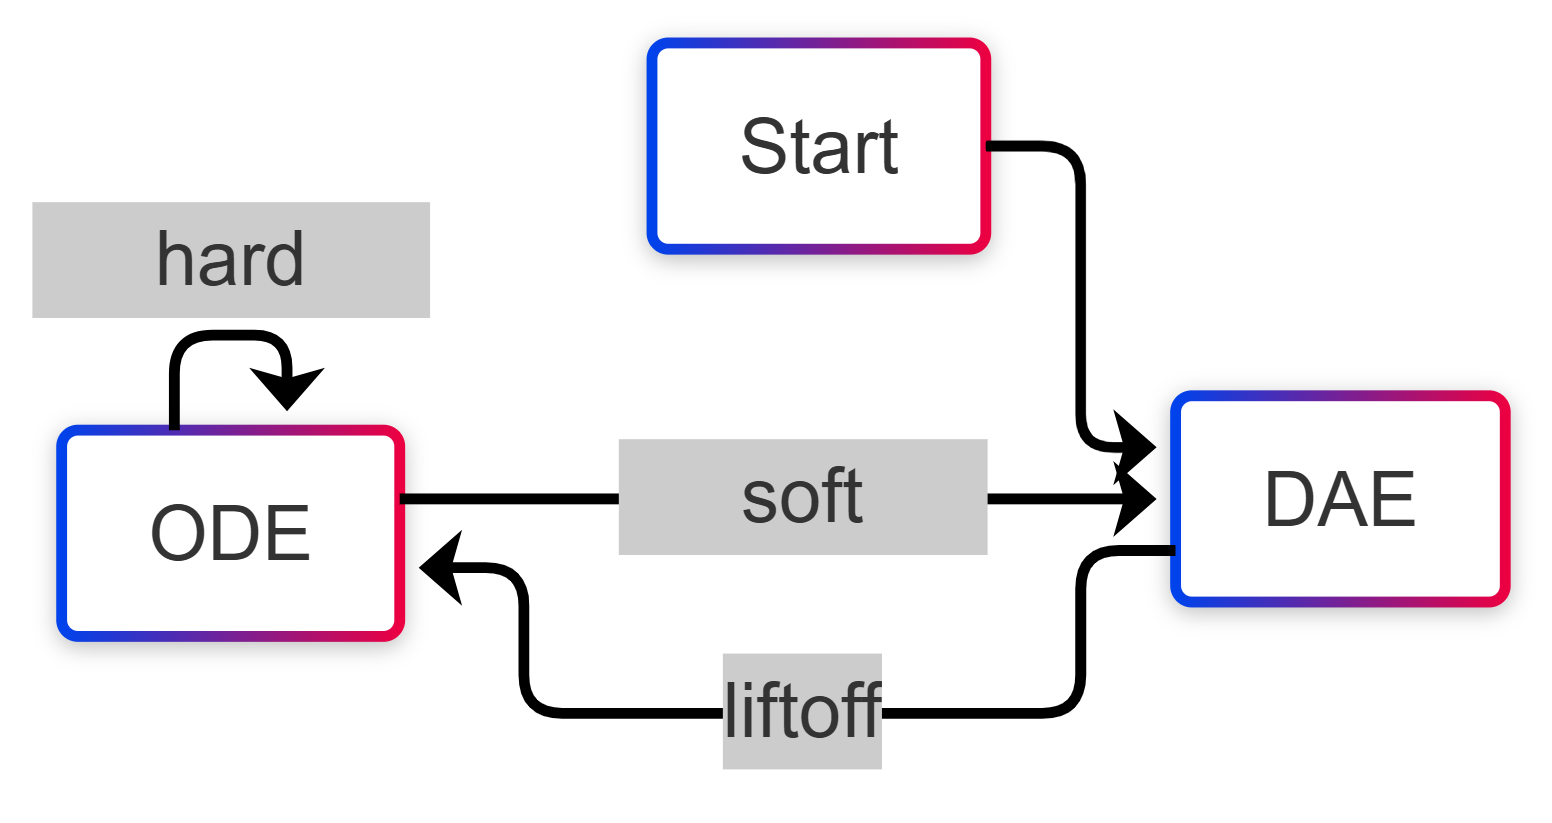
\includegraphics[scale=0.35]{./state_flowchart_2.png}
\end{frame}

\begin{frame}{DAE zu ODE (Ball hebt ab)}
\begin{itemize}
	\item Gesamtkraft in Normalrichtung:
	\[
	F_{\nu} = F_g + F_c
	\]
	mit
	\begin{itemize}
		\item Gravitation in Normalrichtung $F_g = (mg, \nu)$
		\item Zentrifugalkraft $F_c$
	\end{itemize}
	\item Wechsel sobald
	\[
	F_{\nu} < 0
	\]
\end{itemize}
\end{frame}

\begin{frame}{Aufprall auf die Kurve}
	\begin{itemize}
		\item Kurve ist definiert über $G(x) = 0$
		\item Inneres entweder $G(x) < 0$ oder $G(x) > 0$ (konfigurierbar)
		\item Aufprall, wenn $\operatorname{sign}(G(x))$ wechselt
	\end{itemize}
	\pause

	\textbf{Folgen:}
	\begin{itemize}
		\item Projektion der Position $x$ auf Kurve
		\item Zerlegung der Geschwindigkeit in Tangential- und Normalanteil
		\item Dämpfung der Anteile
	\end{itemize}
\end{frame}

\begin{frame}{ODE zu DAE/ODE}
	\textbf{Wechsel zur DAE} (Ball rollt wieder)
	\begin{itemize}
		\item Normalgeschwindigkeit nach Aufprall $<$ Schwelle
		\pause
		\item Normalgeschwindigkeit = 0 gesetzt
		\item Beschleunigung:
		\[
		\mathbf{a}_{DAE} = (\mathbf{a}_{ODE}, \tau) \tau + \kappa \| \mathbf{v}_{DAE} \|^2 \nu
		\]
	\end{itemize}
	\pause
	\textbf{Weiter ODE} (Ball prallt ab)
	\begin{itemize}
		\item Normalgeschwindigkeit $\geq$ Schwelle
		\pause
		\item Normalgeschwindigkeit wird gespiegelt
		\item Beschleunigung bleibt gleich
	\end{itemize}
\end{frame}

\begin{frame}[standout]
	Gibt es Fragen?
\end{frame}


\end{document}
